% -*- coding: utf-8 -*-

\documentclass{beamer}

\usepackage{pri}

\graphicspath{{./}{figures/}{figures/04-classification-figs/}}

\newcommand{\hh}{\hat{h}}
\DeclareMathOperator*{\argmin}{argmin}

\title{Processamento e Recuperação de Informação}

\subtitle{Classification}

\begin{document}

\maketitle
\makeoutline

% ------------------------------------------------------------

\begin{frame}
    \frametitle{Bibliography}
    \begin{block}{}
        \begin{itemize}
        \item \href{https://www.cs.uic.edu/~liub/WebMiningBook.html}{Bing Liu, Web Data Mining - Exploring Hyperlinks, Contents, and Usage Data.} Chapter 3.

        \item \href{http://www.mir2ed.org}{Ricardo Baeza-Yates and Berthier Ribeiro-Neto, Modern Information Retrieval.} Chapter 8.

        \item \href{http://nlp.stanford.edu/IR-book/}{Christopher D. Manning, Prabhakar Raghavan and Hinrich Schütze, Introduction to Information Retrieval.} Chapters 13, 14 and 15.

        \item \href{http://www.mmds.org}{Jure Leskovec, Anand Rajaraman, and Jeff Ullman, Mining of Massive Datasets,} Chapter 12
        \end{itemize}
    \end{block}
\end{frame}

\section{Introduction}

\begin{frame}
  \frametitle{Organizing Knowledge}

  \begin{itemize}
  \item Organize into \emph{systematic knowledge structures}
  \item Ontologies
    \begin{itemize}
    \item \href{https://en.wikipedia.org/wiki/List_of_Dewey_Decimal_classes}{Dewey Decimal System}
    \item \href{http://dl.acm.org/ccs/ccs.cfm}{ACM Computing Classification System}
    \item \href{http://ip-science.thomsonreuters.com/support/patents/dwpiref/reftools/classification/}{Patent Subject Classification}
    \item \href{http://www.who.int/classifications/icd/en/}{International Classification of Diseases}
    \end{itemize}
  \item Web catalogs
    \begin{itemize}
    \item \href{https://en.wikipedia.org/wiki/Yahoo!_Directory}{Yahoo Directory} (RIP 2002--2014)
    \item \href{http://www.dmoz.org/}{DMOZ Directory} (RIP 1998--2017)
    \item \href{http://vlib.org}{World Wide Web Virtual Library}
    \item \href{https://www.jasminedirectory.com}{Jasmine Directory}
    \end{itemize}
  \end{itemize}

  \begin{block}{}<2>
      \centering
      \emph{Problem: Manual maintenance}
  \end{block}

\end{frame}

% ------------------------------------------------------------

\section{Supervised Learning}

\begin{frame}
    \frametitle{Supervised Learning}

    Given a set of \emph{training data} as input, use \emph{learning algorithm}
    $A$ to discover the function $\hh$ that minimizes the \emph{loss} (e.g. the
    error over the set of training instances) %

    \vfill

    \begin{description}
    \item[Input:] $\{(x_i,y_i)\}_{i=1}^N$, $x_i \in \mathcal{R}^M, y_i \in
        \mathcal{R}$
    \item[Hypothesis space:] $h^* \in H$
    \item[Loss function:] $L(h(x),y)$
    \item[Learning Algorithm:] $\hh = A(\{(x_i,y_i)\}_{i=1}^N)$, such that $\hh
        = \argmin_h \sum_{i=1}^N L(h(x_i),y_i)$
    \end{description}
    \vfill
\end{frame}

\begin{frame}
    \frametitle{An Example: Linear Regression}
    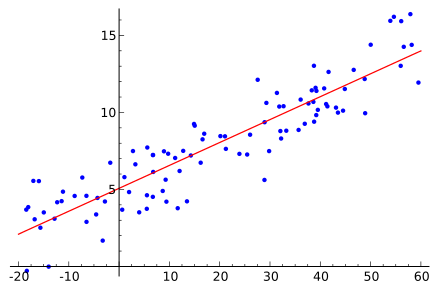
\includegraphics[width=\textwidth]{Linear_regression}\\
    \hfill\footnotesize (source: \href{http://en.wikipedia.org/wiki/Linear_regression}{wikipedia})
\end{frame}

\newcommand{\ww}{\vec{w}}
\begin{frame}
    \frametitle{Linear Regression (cont.)}
    \begin{itemize}
    \item The \emph{hypothesis space}:
        \begin{displaymath}
            h_{\ww}(x) = w_0 + w_1x
        \end{displaymath}
        where $\ww = [w_0, w_1]$
    \item The \emph{loss function}:
        \begin{displaymath}
            L(h_{\ww},y) = \frac{1}{N}\sum_{i=1}^N(y_i - h_{\ww}(x_i))^2
        \end{displaymath}
        i.e. the sum of the squared error
    \item We want to find
        \begin{displaymath}
            w^* = \argmin_w L(h_{\ww},y)
        \end{displaymath}
    \end{itemize}
\end{frame}

\begin{frame}
    \frametitle{Minimizing the Loss}
    \begin{itemize}
    \item In simple cases, we can easily find one (or more) solution(s) to the problem of learning $\hh$
        \begin{itemize}
        \item For linear regression, take the derivatives and equal to $0$
        \end{itemize}
    \item In many cases this is not possible (or we may want to enforce some
        constraints on the parameters) % e.g. como no Lasso ou ridge regression
    \item In practice, there are many ways to estimate $w^*$
    \end{itemize}
\end{frame}

\begin{frame}
    \frametitle{An Example: Gradient Descent}
    \begin{columns}
        \begin{column}{.5\textwidth}
            $w \leftarrow$ any point in the parameter space\\
            \textbf{loop} until convergence \textbf{do}\\
            ~~~~\textbf{for each} $w_i$ \textbf{in} $\ww$ \textbf{do}\\
            ~~~~~~~~$w_i \leftarrow w_i - \alpha\frac{\partial}{\partial w_i}
            L(h_{\ww},y)$\\[\baselineskip]
            $\alpha =$ learning rate
        \end{column}
        \begin{column}{.5\textwidth}
            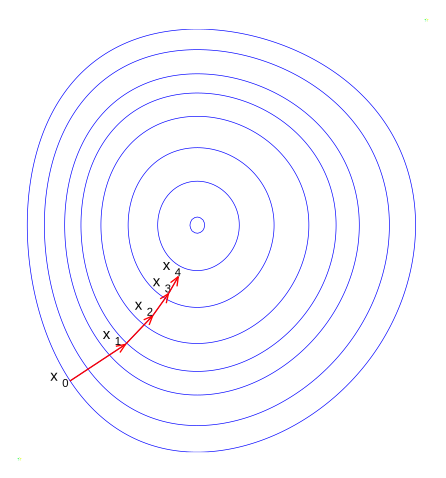
\includegraphics[height=\textwidth]{Gradient_descent}\\
            \hfill\footnotesize (source:
            \href{http://en.wikipedia.org/wiki/Gradient_descent}{wikipedia})
        \end{column}
    \end{columns}
\end{frame}

\begin{frame}
  \frametitle{Classification}

  \begin{itemize}
  \item Learning to assign objects to classes given examples
  \item Learn a \emph{classifier} (i.e., map the problem into supervised learning task)
  \end{itemize}

  \vspace{5ex}

  \centering
  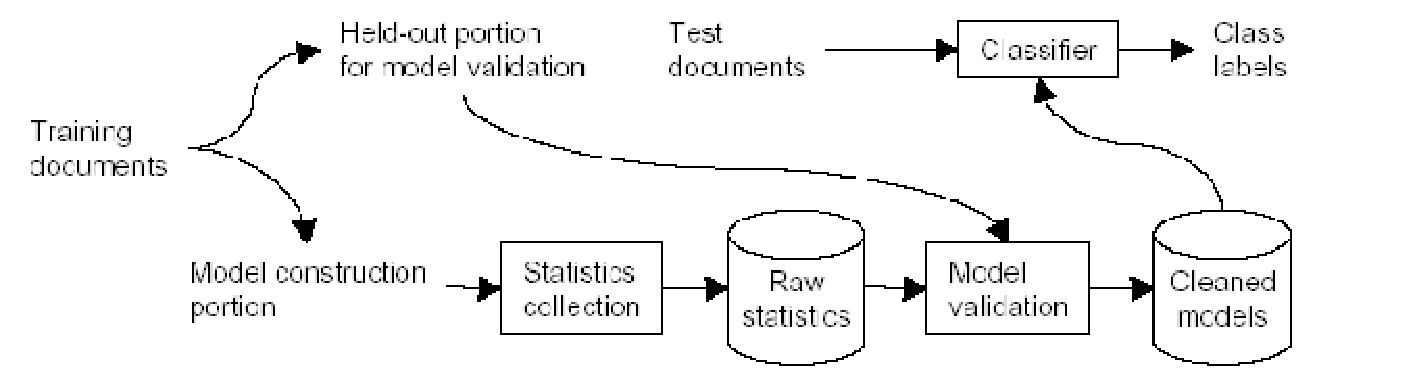
\includegraphics[width=\linewidth]{learning}

\end{frame}

\begin{frame}
    \frametitle{An Example: Logistic Regression}

    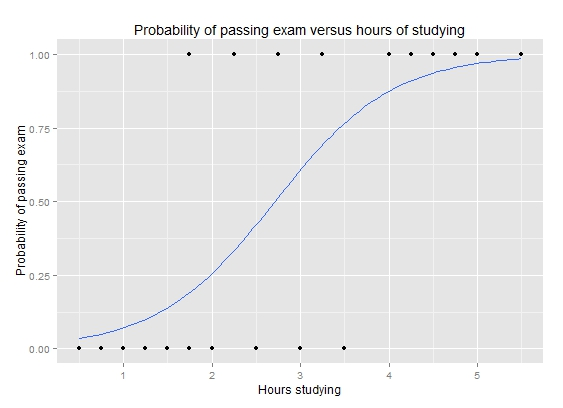
\includegraphics[width=.9\textwidth]{Exam_pass_logistic_curve}\\
    \hfill\footnotesize (source: \href{https://en.wikipedia.org/wiki/Logistic_regression}{wikipedia})
\end{frame}

\begin{frame}
    \frametitle{Logistic Regression (cont.)}
    \begin{itemize}
    \item The \emph{hypothesis space}:
        \begin{displaymath}
            h_{\ww}(x) = \frac{1}{1 + e^{-(w_0 + w_1x)}}
        \end{displaymath}
        where $\ww = [w_0, w_1]$
    \item The \emph{loss function}:
        \begin{displaymath}
            L(h_{\ww},y) = \frac{1}{N}\sum_{i=1}^NC(h_{\ww}(x_i),y)
        \end{displaymath}
        where
        \begin{displaymath}
            C(h_{\ww}(x),y) =
            \begin{cases}
                -\log(h_{\ww}(x)) & \text{if $y=1$} \\
                -\log(1 - h_{\ww}(x)) & \text{if $y=0$}
            \end{cases}
        \end{displaymath}
    \item We want to find
        \begin{displaymath}
            w^* = \argmin_w L(h_{\ww},y)
        \end{displaymath}
    \end{itemize}
\end{frame}

% https://towardsdatascience.com/logistic-regression-detailed-overview-46c4da4303bc
% https://ml-cheatsheet.readthedocs.io/

% ------------------------------------------------------------

\section{Text Classifiers}

% ------------------------------------------------------------

\begin{frame}
  \frametitle{Text Classification vs. Data Mining}
  \begin{block}{}
  Leverage supervised learning together with method for representing textual information (e.g., VSM with TF-IDF)
  \end{block}
  
  \begin{itemize}
  \item Lots of features and a lot of noise
  \item No fixed number of columns
  \item No categorical attribute values
  \item Data scarcity
  \item Larger number of class labels
  \item Hierarchical relationships between classes less systematic
  \end{itemize}

\end{frame}

% ------------------------------------------------------------

\begin{frame}
  \frametitle{Text Classifiers}

  \begin{itemize}
  \item Nearest Neighbor Classifiers
    \begin{itemize}
    \item Classify documents according to the class distribution of their neighbors
    \end{itemize}
  \item Generative Bayesian classifiers (e.g., na{\"i}ve Bayes)
    \begin{itemize}
    \item Discover the class distribution most likely to have generated a test
      document
    \end{itemize}
  \item Linear discriminative classifiers (e.g., the perceptron, logistic regression, or support vector machines):
    \begin{itemize}
    \item Discover an hyperplane that separates classes
    \end{itemize}
  % \item Rule induction:
  %   \begin{itemize}
  %   \item Induce rules for classification over diverse features
  %   \end{itemize}
  \item Neural networks
    \begin{itemize}
    \item Discover a non-linear function, often resulting from a composition of many functions, that separates classes
    \end{itemize}    
  \end{itemize}

\end{frame}

\subsection{Nearest Neighbor Classifiers}

\begin{frame}
  \frametitle{Nearest Neighbor Classifiers}

  \begin{itemize}
  \item Intuition: similar documents are expected to be assigned the same class label
    \begin{itemize}
    \item Similarity: vector space model + cosine similarity
    \end{itemize}
  \item Training:
    \begin{itemize}
    \item Index each document and remember class label
    \end{itemize}
  \item Testing:
    \begin{itemize}
    \item Fetch \emph{$k$ most similar} documents to the given document
    \item Majority class wins
    \item Alternatives:
      \begin{itemize}
      \item Weighted counts: counts of classes weighted by the corresponding
        similarity measure
      \item Per-class offset: tuned by testing the classifier on a portion of
        training data held out for this purpose
      \end{itemize}
    \end{itemize}
  \end{itemize}

\end{frame}

% ------------------------------------------------------------

\begin{frame}
  \frametitle{$k$NN Classifier}

  \centering
  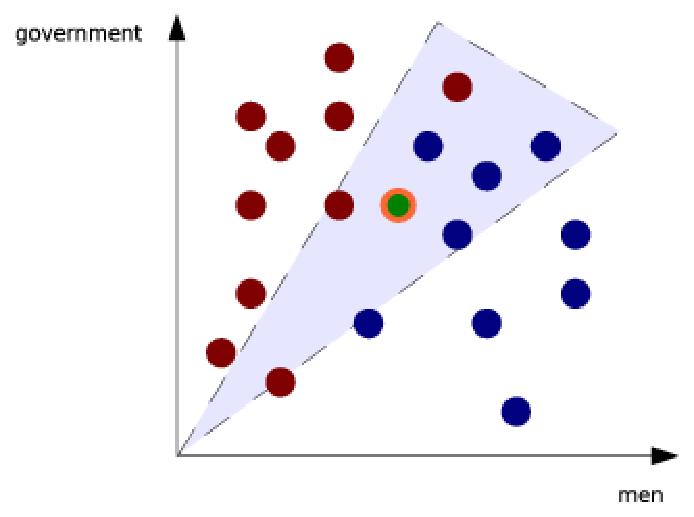
\includegraphics[width=.7\linewidth]{knn}
  \begin{displaymath}
    score(c,d_q) = b_c + \sum_{d \in kNN(d_q)}sim(d_q,d)
  \end{displaymath}

\end{frame}

% ------------------------------------------------------------

\begin{frame}
  \frametitle{Properties of $k$NN}

  \begin{itemize}
  \item Advantages:
        \begin{itemize}
        \item Reuse of standard vector space model and availability of associated technology (e.g., inverted indexes)
        \item Collection updates are trivial
        \item Accuracy comparable to best known classifiers
        \end{itemize}
  \item<+-> Problems:
        \begin{itemize}
        \item Classification efficiency
            \begin{itemize}
            \item many lookups over the document collection/index
            \item sorting by overall similarity
            \item picking the best $k$ documents
            \end{itemize}
        \item Space overhead and redundancy
             \begin{itemize}
             \item Data stored at level of individual documents
             \item Poor generalization
             \end{itemize}
        \item Choosing a value for $k$
        \end{itemize}
  \end{itemize}

\end{frame}

% % ------------------------------------------------------------

\begin{frame}
  \frametitle{Improvements for $k$NN}

  \begin{itemize}
  \item To reduce space requirements and speed up classification
    \begin{itemize}
    \item Find clusters in the data and start by comparing instances against clusters \emph{(clustering covered in the next lecture)}
    \item Store only a few statistical parameters per cluster
    \item In second step, compare with documents in only the most promising clusters
    \end{itemize}
  \item However...
    \begin{itemize}
    \item Ad-hoc choices for number and size of clusters and parameters
    \item Number of clusters depends on the data
    \end{itemize}
  \end{itemize}

\end{frame}

% ------------------------------------------------------------

\subsection{Generative Bayesian Classifiers}

\begin{frame} \frametitle{Bayesian Classifiers}
  
  \begin{itemize}
  \item Probabilistic document classifier
  \item Assumptions:
    \begin{enumerate}
    \item A document can belong to \emph{exactly one class}
    \item Each class $c$ has an associated prior probability $P(c)$
    \item There is a class-conditional document distribution $P(d|c)$ for each
      class (i.e., the likelihood)
    \end{enumerate}
  \item Given a document $d$, the probability of it being generated by class
    $c$ is:
    \begin{displaymath}
      P(c|d) = \frac{P(d|c)P(c)}{\sum_{\gamma}P(d|\gamma)P(\gamma)}
    \end{displaymath}
  \item The class with the highest probability is assigned to $d_q$ (i.e., we use a {\it maximum a-posteriory} rule)
  \end{itemize}

\end{frame}

% ------------------------------------------------------------

\begin{frame} \frametitle{Learning the Document Distribution}
  
  \begin{itemize}
  \item $P(d|c)$ is estimated based on parameters $\Theta$
  \item $\Theta$ are estimated based on two factors:
    \begin{enumerate}
    \item Prior knowledge before seeing any documents
    \item Terms in the training documents
    \end{enumerate}
  \item Bayes Optimal Classifier
    \begin{displaymath}
      P(c|d) = \int_\Theta\frac{P(d|c,\Theta)P(c|\Theta)}
      {\sum_{\gamma}P(d|\gamma,\Theta)P(\gamma|\Theta)} P(\Theta|D)
    \end{displaymath}
    \begin{itemize}
    \item This can be hard to compute
    \end{itemize}
  \item Maximum Likelihood Estimate: $P(d|c, \hat{\Theta})$
    \begin{displaymath}
        \hat{\Theta} = argmax_\Theta P(d|c,\Theta)
    \end{displaymath}
    %\item Replace the marginal with the value of $P(d|c,\Theta)$ for
    %    $argmax_\Theta P(\Theta|D)$
  \end{itemize}

\end{frame}

% ------------------------------------------------------------

\begin{frame} \frametitle{Na{\"i}ve Bayes Classifier}
  
  \begin{itemize}
  \item Na{\"i}ve assumption
    \begin{itemize}
    \item assumption of \emph{independence between terms}
    \item joint term distribution is the product of the marginals
    \end{itemize}
  \item Widely used owing to
    \begin{itemize}
    \item simplicity and speed of training, applying, and updating
    \end{itemize}
  \item Two kinds of widely used marginals for text
    \begin{itemize}
    \item Binary model (Bernoulli)
    \item Multinomial model
    \end{itemize}
  \end{itemize}

\end{frame}

% ------------------------------------------------------------

\begin{frame} \frametitle{Na{\"i}ve Bayes Models}

    \emph{Binary Model:}  % bernoulli
    Each parameter $\theta_{c,t}$ indicates the probability that a document in class $c$ will mention term $t$ at least once

    \begin{displaymath}
        P(d|c,\Theta) = \Pi_{t \in d}\theta_{c,t} \Pi_{t \not\in d}(1-\theta_{c,t})
    \end{displaymath}
    \begin{displaymath}
        \theta_{c,t} = \frac{N_{c,t}}{N_c}
    \end{displaymath}
    $N_{c,t} =$ n. of docs in class $c$ containing term $t$\\
    $N_c = $ n. of docs in class $c$
\end{frame}

\begin{frame} \frametitle{Na{\"i}ve Bayes Models (cont.)}

  \emph{Multinomial Model:}  % multinomial
  \begin{itemize}
  \item each class has an associated die with $|W|$ faces
  \item each parameter $\theta_{c,t}$ denotes probability of the face turning
    up on tossing the die, i.e. $\sum_{d \in c}n(d,t) / \sum_{d \in c}\ell_d$
  \item term $t$ occurs $n(d,t)$ times in document $d$
  \item document length is a random variable denoted $L$
  \end{itemize}
  \begin{displaymath}
    \begin{split}
          P(d|c,\Theta) & = P(L = \ell_d|c)P(d|\ell_d,c) \\
                  & = P(L = \ell_d|c)
                      \frac{\ell_d!}{\Pi_{t \in d}n(d,t)!}
                      \Pi_{t \in d}\theta_{c,t}^{n(d,t)} \\
                 & \sim P(L = \ell_d|c)
                     \Pi_{t \in d}\theta_{c,t}^{n(d,t)}
    \end{split}
   \end{displaymath}

\end{frame}

% ------------------------------------------------------------

\begin{frame} \frametitle{Parameter Smoothing}
  
  \begin{itemize}
  \item What if a test document $d_q$ contains a term $t$ that never occurred
      in any training document in class $c$?
      \pause
    \begin{itemize}
    \item $P(c|d_q) = 0$
    \item Even if many other terms clearly hint at a high likelihood of class
      $c$ generating the document
    \end{itemize}
  \item Thus, MLE cannot be used directly
  \item We can use \emph{Laplace smoothing}
    \begin{itemize}
    \item Simply adds 1 to each count
    \end{itemize}
    \begin{displaymath}
        \theta_{c,t} = \frac{\sum_{d \in c}n(d,t) + 1}{\sum_{d \in c}\ell_d + |W|}
        %\frac{n(c,t) + 1}{\sum_{t \in W}n(c,t) + |W|}
    \end{displaymath}
  \end{itemize}

\end{frame}

% % ------------------------------------------------------------

% \begin{frame} \frametitle{Laplace's Law of Succession}
  
%   \begin{itemize}
%   \item The estimate $\tilde{\theta}$ is usually a property of the posterior
%     distribution $\pi(\theta|\langle k,n \rangle)$
%   \item We define a \emph{loss function}
%     \begin{itemize}
%     \item Penalty for picking a smoothed value against the \textit{true} value
%     \end{itemize}
%   \item For the loss function 
%     \begin{displaymath}
%       L(\theta,\tilde{\theta}) = (\theta - \tilde{\theta})^2
%     \end{displaymath}
%     the appropriate estimate to use is the expectation $E(\pi(\theta|\langle
%     k,n \rangle))$
%   \item This yields
%     \begin{displaymath}
%       \tilde{\theta} = \frac{k + 1}{n + 2}
%     \end{displaymath}
%   \end{itemize}

% \end{frame}

% ------------------------------------------------------------

\begin{frame} \frametitle{Performance Analysis}
  
  \begin{itemize}
  \item Multinomial na{\"i}ve Bayes classifier generally outperforms the binary
    variant
  \item $k$NN may outperform Na{\"i}ve Bayes
  \item Na{\"i}ve Bayes is faster and more compact
  \item Determines \emph{decision boundaries}
    \begin{itemize}
    \item Regions of the term-space where different classes have similar
      probabilities
    \item Documents in these regions are hard to classify
    \item Strongly biased
    \end{itemize}
  \end{itemize}

\end{frame}

% \begin{frame} \frametitle{Na{\"i}ve Bayes and the LM-Based Retrieval Approach}
    
%     \begin{block}{}
%     The previous lectures introduced a simple probabilistic model for {\it ad-hoc} document retrieval, based on language modeling
%     \end{block}
  
%     \scriptsize
%     \begin{itemize}
%     \item We want to classify document $d$. \\ \emph{We want to classify a query $q$}
% 	\item Human-defined classes: e.g., politics, economics, sports. \\ \emph{Each document in the collection is a different class}
% 	\item Assume that $d$ was produced by the generative model. \\ \emph{Assume that $q$ was generated by a generative model}
%     \item Which of the classes (= class models) is most likely to have generated the document $d$? \\ \emph{Which document (=class) is most likely to have generated the query $q$?}
%     \item For which class do we have the most evidence? \\ \emph{For which document (as source for query) do we have the most evidence?}
% 	\end{itemize}

% \end{frame}

% ------------------------------------------------------------

\subsection{Linear Discriminative Classifiers}

\begin{frame} \frametitle{Discriminative Classification}

  \begin{itemize}
  \item Na{\"i}ve Bayes classifiers are \emph{generative}
  \item Differently, \emph{discriminative} classifiers:
    \begin{itemize}
    \item Directly map the feature space to class labels
    \item Class labels are encoded as numbers
      \begin{itemize}
      \item e.g: +1 and -1 for two a class problem
      \end{itemize}
    \end{itemize}
  \item For instance, we can try to find a vector $\alpha$ such that the sign
    of $\alpha \cdot d + b$ directly predicts the class of a document $d$
  \item Possible solutions:
    \begin{itemize}
    \item Linear least-square regression
    \item \emph{The Perceptron}
    \item \emph{Logistic Regression}
    \item \emph{Support Vector Machines}
    \end{itemize}
  \end{itemize}
  
\end{frame}

% ------------------------------------------------------------

\begin{frame} \frametitle{What is a Linear Discriminative Classifier?}
  \begin{itemize}
  \item Essentially:
    \begin{itemize}
    \item Classification decision is based on the value of a linear combination of the features
    \item Can be seen as the splitting of a high-dimensional input space with a hyperplane
    \end{itemize}
  \end{itemize}
  \begin{equation*}
    y(d_1,\ldots,d_n) = f(\alpha_1d_1 + \alpha_2d_2 + \ldots + \alpha_nd_n)
  \end{equation*}
  \begin{itemize}
    \item $\alpha_i$ are parameters (i.e., the weight of each feature $d_i$)
    \item $f$ is the activation function (e.g., $f(d) = 1_{x \geq 0}(d)$)
    \item The result of $y(d_1,\ldots,d_n)$ corresponds to the estimated class
  \end{itemize}
\end{frame}

\begin{frame} \frametitle{The Bias Term}
  \begin{itemize}
  \item Notice that, according to the previous definition, the decision hyperplane must go through the origin
  \item Could be achieved by preprocessing the input, but this is not always desirable or possible
  \item Solution : Add a bias input:
  \begin{equation*}
    y(d_1,\ldots,d_n) = f(b + \alpha_1d_1 + \ldots + \alpha_nd_n)
  \end{equation*}
  \item Same as an input connected to the constant $1$
  \item We consider this {\it ghost} input implicit henceforth
  \end{itemize}
\end{frame}

\begin{frame} \frametitle{Training : The Perceptron Algorithm}
    \begin{itemize}
    \item Switching to vector notation:
        \begin{equation}
            y(\mathbf d) = f(\mathbf \alpha \mathbf d) = f_{\mathbf \alpha}(d)
        \end{equation}
    \item Assume we need to separate sets of points $A$ (i.e., the positive examples) and $B$ (i.e., the negative examples)
        \begin{equation}
            E(\mathbf \alpha) = \displaystyle\sum_{\mathbf d\in A}(1 - f_{\mathbf \alpha}(\mathbf d)) + \displaystyle\sum_{\mathbf d\in B}f_{\mathbf \alpha}(\mathbf d)
        \end{equation}
    \item Goal: $E(\mathbf \alpha) = 0$
    \item Start from a random $\mathbf \alpha$ and improve it iteratively
    \end{itemize}
\end{frame}

\begin{frame} \frametitle{Algorithm Pseudo-Code}
    \begin{enumerate}
    \item Start with random $\mathbf \alpha$, set $t = 0$
    \item Select a vector $\mathbf d \in A \cup B$
    \item If $\mathbf d \in A$ and $\mathbf \alpha \mathbf d \leq 0$, then $\mathbf \alpha_{t+1} = \mathbf \alpha_t + \mathbf d$
    \item Else if $\mathbf d \in B$ and $\mathbf \alpha \mathbf d \geq 0$, then $\mathbf \alpha_{t+1} = \mathbf \alpha_t - \mathbf d$    
    \item Conditionally go to step 2
    \end{enumerate}
    \begin{itemize}
    \item Guaranteed to converge \emph{iff} $A$ and $B$ are linearly separable!
    \end{itemize}
\end{frame}

\begin{frame} \frametitle{Problems of Simple Perceptrons (1)}
\begin{block}{Overfitting}
\begin{itemize}
\item The standard Perceptron returns the most recent version of the weight vector
\item Intuitively, this version is over-adapted to the last few instances, and may work less well for other instances
\end{itemize}
\end{block}
\begin{block}{}
\begin{itemize}
\item The \emph{Averaged Perceptron} returns the average of all versions (or the last few versions) of the weight vector
\item An implementation trick involves setting a learning step that takes the averaging effect into account
\end{itemize}
\end{block}
\end{frame}

\begin{frame} \frametitle{Problems of Simple Perceptrons (2)}
\begin{block}{Multi-class classification}
\begin{itemize}
\item Several problems involve \emph{multi-class classification}
\item Multi-class classification can be made through one weight vector for each category, assigning instances to the class for which the model predicts a higher value
\end{itemize}
\end{block}
\begin{block}{}
\begin{itemize}
\item In practice, we can represent this with one giant weight vector and repeated features for each category
\item Update rule involves changing the weights for the true class and the class that was predicted
\item Other options for update rule can be considered, e.g. updating classes with higher score than correct one 
\end{itemize}
\end{block}
\end{frame}

\begin{frame} \frametitle{Summary of Simple/Averaged Perceptrons}
  \begin{itemize}
  \item Simple and reasonably efficient online training
  \item Easy to extend in order to consider multi-class classification (and also structured prediction)
  \item Works well for document classification, and more generally for problems with many features
  \item Limited capabilities (e.g., does not try to optimize the separation ``distance'' between classes)
  \begin{itemize}
  \item Just looks for a hyperplane that separates the two sets 
  \item Methods such as \emph{Support Vector Machines}, on the other hand, try to maximize the distance between two closest opposite sample points (i.e., the \emph{margin of the separating hyperplane} between the classes)
  \end{itemize}  
  \end{itemize}
\end{frame}

% ------------------------------------------------------------

\begin{frame} \frametitle{Linear Discriminative Classifiers and SVMs}
  
  \begin{itemize}
%  \item Assumption: training and test population are drawn from the same distribution
  \item Hypothesis:
    \begin{itemize}
    \item The classes can be separated by an \emph{hyperplane}
    \item The hyperplane that is close to many training data points has a greater chance of misclassifying test instances
    \item An hyperplane that passes through a "no-man's land", has lower chances of misclassifications
    \end{itemize}
  \item Make a decision by thresholding
    \begin{itemize}
    \item Seek an hyperplane that maximizes the distance to any training point
    \item Choose the class on the same side of the hyperplane as the test
      document (i.e., same as in the Perceptron)
    \end{itemize}
  \end{itemize}

\end{frame}

% ------------------------------------------------------------

\begin{frame} \frametitle{Discovering the Hyperplane}
  
  \begin{itemize}
  \item Assume the training documents are separable by an hyperplane
    perpendicular to a vector $\alpha$
  \item Seek a vector $\alpha$ which maximizes the distance of any training point to
    the hyperplane
  \item This corresponds to solving the following \emph{quadratic programming} problem:
    \begin{displaymath}
      \begin{array}{rl}
        \text{Minimize} & \frac{1}{2}\alpha\cdot\alpha \\
        \text{subject to} & c_i(\alpha\cdot d_i + b) \geq 1, \forall i = 1,
        \dotsc, n
      \end{array}
    \end{displaymath}
  \end{itemize}

\end{frame}

% ------------------------------------------------------------

\begin{frame} \frametitle{SVM Classifier}

  \centering
  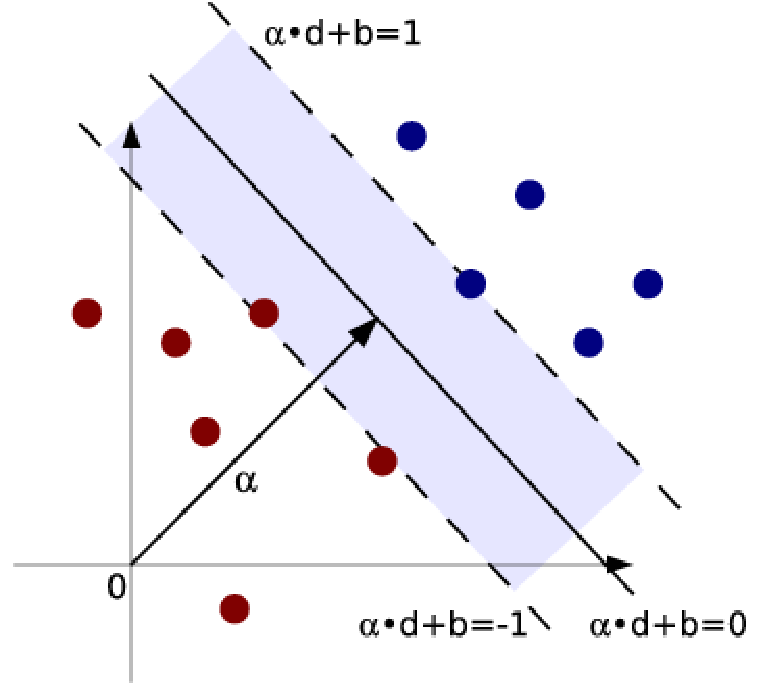
\includegraphics[width=.7\linewidth]{svm}

\end{frame}

% ------------------------------------------------------------

\begin{frame} \frametitle{Non Separable Classes}
  
  \begin{itemize}
  \item Classes in the training data not always separable
  \item We introduce \emph{slack variables}
    \begin{displaymath}
      \begin{array}{rl}
        \text{Minimize} & \frac{1}{2}\alpha\cdot\alpha + C\sum_i\xi_i \\
        \text{subject to} & c_i(\alpha\cdot d_i + b) \geq 1 - \xi_i,
        \forall i = 1, \dotsc, n \\
        \text{and} & \xi_i \geq 0, \forall i = 1, \dotsc, n 
      \end{array}
    \end{displaymath}
  \item Implementations often solve the equivalent dual problem
     \begin{displaymath}
      \begin{array}{rl}
         \text{Maximize} & \sum_i\lambda_i - \frac{1}{2}\sum_{i,j}\lambda_i\lambda_j c_i c_j (d_i \cdot d_j) \\
         \text{subject to} & \sum_i c_i\lambda_i = 0 \\
         \text{and} & 0 \leq \lambda_i \leq C, \forall i=1, \dotsc, n
      \end{array}
     \end{displaymath}
  \end{itemize}

\end{frame}

% ------------------------------------------------------------

\begin{frame} \frametitle{Analysis of SVMs}
  
  \begin{itemize}
  \item Complexity:
    \begin{itemize}
    \item Quadratic optimization problem
    \item Requires on-demand computation of inner-products
    \item Recent SVM packages work in linear time
    \end{itemize}
  \item Performance:
    \begin{itemize}
    \item Amongst most accurate classifier for text
    \item Better accuracy than Na{\"i}ve Bayes and most classifiers
    \item Linear SVMs suffice
      \begin{itemize}
      \item Standard text classification tasks have classes almost separable
        using a hyperplane in feature space
      \end{itemize}
    \item Non-linear SVMs can be achieved through \emph{kernel functions}
    \end{itemize}
  \end{itemize}

\end{frame}

\begin{frame} \frametitle{Logistic Regression as a Linear Classifier}
Recall that for logistic regression, we have that:

\begin{center}
a
\end{center}

We would predict positive if $P(Y=1|X)>P(Y=0|X)$, or equivalently:

\begin{center}
\begin{equation}
\frac{P(Y=1|X)}{P(Y=0|X)} > 1
\end{equation}
\end{center}

Taking logs on both sides:

\begin{center}
\begin{equation}
\log \left( \frac{P(Y=1|X)}{P(Y=0|X)} \right) > 0
\end{equation}
\end{center}

Thus, we see that the decision boundary is given by the plane $w_0 +_sum_i w_i \dot X_i$ (similarly to the Perceptron or SVM classifiers).
\end{frame}


%\section{Evaluation of Classifiers}

%\subsection{Single-Class Classifiers}

%\begin{frame} \frametitle{Measures of Accuracy}
  
%  Two cases:
%  \begin{enumerate}
%  \item Each document is associated with exactly \emph{one class}, or
%  \item Each document is associated with a \emph{subset of classes}
%  \end{enumerate}

%\end{frame}

% ------------------------------------------------------------

%\begin{frame} \frametitle{Single-class Scenario}
  
%  \begin{itemize}
%  \item For the first case, we can use a \emph{confusion matrix} $M$
%    \begin{itemize}
%    \item $M[i,j]$ is the number of test documents belonging to class $i$ which
%      were assigned to class $j$
%    \item Perfect classifier: diagonal elements $M[i,i]$ would be nonzero
%    \item Example:
%      \begin{displaymath}
%        \footnotesize
%        M = \left\{
%          \begin{array}{c|c|c}
%            5 & 0 & 0 \\\hline
%            1 & 3 & 0 \\\hline
%            1 & 2 & 4
%          \end{array}
%        \right\}
%      \end{displaymath}
%    \end{itemize}
%  \item If $M$ is large, we use
%    \begin{displaymath}
%      \text{accuracy} = \sum_i M[i,i] / \sum_{i,j} M[i,j]
%    \end{displaymath}
%  \end{itemize}

%\end{frame}

% ------------------------------------------------------------

%\subsection{Multiple-Class Classifiers}

%\begin{frame} \frametitle{Multiple-class Scenario}
  
%  \begin{itemize}
%  \item One-vs.-rest
%    \begin{itemize}
%    \item Create a two-class problem for every class
%      \begin{itemize}
%      \item E.g. ``sports'' and ``not-sports'', ``science'' and
%        ``not-science'', etc.
%      \end{itemize}
%    \item We have a classifier for each case
%    \end{itemize}
%  \item Accuracy is measured by \emph{recall} and \emph{precision}
%    \begin{itemize}
%    \item Let $C_d$ be the correct classes for document $d$ and $C'_d$ be the
%      set of classes estimated by the classifier
%      \begin{displaymath}
%        precision = \frac{C'_d \cap C_d}{C'_d}
%      \end{displaymath}
%      \begin{displaymath}
%        recall = \frac{C'_d \cap C_d}{C_d}
%      \end{displaymath}
%    \end{itemize}
%  \end{itemize}
%\end{frame}

% ------------------------------------------------------------

%\begin{frame} \frametitle{Micro-Averaged Precision}
  
%  In a problem with $n$ classes, let $C_i$ be the number of documents in class
%  $i$ and let $C'_i$ be the number of documents estimated to be of class $i$ by
%  the classifier
%  \begin{itemize}
%  \item \emph{Micro-averaged precision} is defined as
%    \begin{displaymath}
%      \frac{\sum_{i=1}^n C'_i \cap C_i}{\sum_{i=1}^n C'_i}
%    \end{displaymath}
%  \item \emph{Micro-averaged recall} is defined as
%    \begin{displaymath}
%      \frac{\sum_{i=1}^n C'_i \cap C_i}{\sum_{i=1}^n C_i}
%    \end{displaymath}
%  \end{itemize}
%
%  \begin{itemize}
%  \item Micro-averaged precision/recall measures correctly classified
%    documents, thus favoring large classes
%  \end{itemize}
%\end{frame}

% ------------------------------------------------------------

%\begin{frame} \frametitle{Macro-Averaged Precision}
  
%  In a problem with $n$ classes, let $P_i$ and $R_i$ be the precision and
%  recall, respectively, achieved by a classifier for class $i$
%  \begin{itemize}
%  \item \emph{Macro-averaged precision} is defined as
%    \begin{displaymath}
%      \frac{1}{n}\sum_{i=1}^n P_n
%    \end{displaymath}
%  \item \emph{Macro-averaged recall} is defined as
%    \begin{displaymath}
%      \frac{1}{n}\sum_{i=1}^n R_n
%    \end{displaymath}
%  \end{itemize}

%  \begin{itemize}
%  \item Macro-averaged precision/recall measures performance per class, giving
%    all classes equal importance
%  \end{itemize}
%\end{frame}

% ------------------------------------------------------------

% \subsection{Other Measures}

% \begin{frame} \frametitle{Other Measures}
  
%   \begin{itemize}
%   \item \emph{Precision-recall graphs}
%     \begin{itemize}
%     \item Show the tradeoff between precision and recall
%     \end{itemize}
%   \item \emph{Break-even point}
%     \begin{itemize}
%     \item Point in the precision/recall graph where precision equals recall
%     \end{itemize}
%   \item The \emph{$F_1$ measure}
%     \begin{displaymath}
%       F_1 = \frac{2 \times P_i \times R_i}{P_i + R_i}
%     \end{displaymath}
%     \begin{itemize}
%     \item Harmonic mean between precision and recall
%     \item Discourages classifiers that trade one for the other
%     \end{itemize}
%   \end{itemize}

% \end{frame}

% ------------------------------------------------------------

\subsection{Neural Networks}

\begin{frame}
    \frametitle{Neural Networks}
\end{frame}

% ------------------------------------------------------------

\section{Other Issues}

\begin{frame}
    \frametitle{Other Issues (1)}

    \begin{itemize}
    \item Tokenization and feature extraction
        \begin{itemize}
        \item E.g.: replacing monetary amounts by a special token, part-of-speech tagging, representations based on $n$-grams, etc.
        \end{itemize}
    
    \item Handling scenarios with multiple classes, or with multiple labels per test document, with binary classifyers like SVMs
        \begin{itemize}
        \item E.g., one-vs.-rest heuristic
            \begin{itemize}
            \item {\scriptsize ~~~~ e.g. ``sports'' vs. ``not-sports'', ``science'' vs.
                  ``not-science'', etc.}
            \item Create a classifier for each case
            \item Assign class(es) with the highest confidence
            \end{itemize}
        \end{itemize}
    \end{itemize}
\end{frame}

\begin{frame}
  \frametitle{Other Issues (2)}
  
  \begin{itemize}
  \item Evaluating text classifiers
    \begin{itemize}
    \item Accuracy
    \item Training speed and scalability
    \item Simplicity, speed, and scalability for document modifications
    \item Ease of diagnosis, interpretation of results, and adding human
      judgment and feedback
    \end{itemize}
  \end{itemize}
  \begin{itemize}
  \item Many other practical issues...
  \end{itemize}
\end{frame}

% ------------------------------------------------------------

\finalframe{Questions?}

\end{document}
